\documentclass[9pt,twocolumn,twoside]{gsajnl}
% Use the documentclass option 'lineno' to view line numbers

\articletype{inv} % article type
% {inv} Investigation 
% {gs} Genomic Selection
% {goi} Genetics of Immunity 
% {gos} Genetics of Sex 
% {mp} Multiparental Populations

\title{Analysis of a The Cancer Genome Atlas (TCGA) RNA-seq data set on Uterine Corpus Endometrial Carcinoma (UCEC)}

\author[$\ast$]{Aguirre, J.}
\author[$\ast$]{Funosas, G.}
\author[$\ast$,1]{Prat, C.}

\affil[$\ast$]{University Pompeu Fabra}

\keywords{UCEC; TCGA; RNA-seq; Differential Expression; Functional Enrichment;}

\runningtitle{GENETICS | Investigation} % For use in the footer 

\correspondingauthor{Joaquim Aguirre, Gerard Funosas, Cristina Prat}

\begin{abstract}
The Cancer Genome Atlas (TCGA) focuses on finding the genetic bases of cancer in human (\textit{Homo sapiens sapiens}) different tissues. The RNA sequencing tool provides information of the transcriptome of a biological sample in a given condition. Comparing tumorous and healthy samples, the differences in gene expression between those conditions can be uncovered. Uterine Corpus Endometrial Carcinoma (UCEC) is one of the most common cancers within women. In this study, a uterine RNA-seq dataset from TCGA has been analysed using bioinformatic tools. A paired sample sub-setting and a low-expressed genes filtering left a quality-filtered dataset of 11571 genes for 32 paired samples. After fitting the data in a regression linear model, taking into account both a surrogate variable analysis and one known covariate effect, the number of differentially expressed genes summed 7845 (68\%). The corresponding GO terms for each of those genes was assigned, and the most represented biological processes in the whole dataset were obtained and ordered by significance.  8 out of the 10 functional groups most differentially expressed in tumorous samples were related to cancer biochemical processes, such as tissue growth, immune response or cell signaling pathways. Another one was directly related to uterine muscle contraction, altered by cancer. Those results show that, even if the genetic bases of cancer are complex, there are both universal patterns in multiple kinds of cancer and specific ones for specific tumor types that can be further assessed to find new ways of controlling tumor development.
\end{abstract}

\setboolean{displaycopyright}{true}

\begin{document}

\maketitle
\thispagestyle{firststyle}
\marginmark
\firstpagefootnote
\correspondingauthoraffiliation{cristina.prat.ferrer@gmail.com}
\vspace{-11pt}%


\section*{Introduction}

Endometrial cancer develops in the cells that form the inner lining of the uterus, or the endometrium, and is one of the most common cancers of the female reproductive system. In 2010, approximately 43,000 women in the United States were estimated to have been diagnosed and almost 8,000 to have died of endometrial cancer. This cancer occurs most commonly in women aged 60 years or older. About 69 percent of endometrial cancers are diagnosed at an early stage, and as a result about 83 percent of women will survive five years following the time of diagnosis.\\
\newline
\href{http://cancergenome.nih.gov/cancersselected/endometrial}{The Cancer Genome Atlas} (TCGA) researchers have:
\begin{itemize}
\item Identified four subtypes of endometrial cancer: POLE ultramutated, Microsatellite instability hypermutated, Copy number low and Copy number high.
\item Uncovered shared genomic features between endometrial cancer and serous ovarian cancer, the Basal-like subtype of breast cancer as well as colorectal cancer.
\item Identified three histologic diagnosis: Endometrioid endometrial adenocarcinoma, Mixed serous and endometrioid and Serous endometrial adenocarcinoma
\item Characterized the marked differences between the two types of endometrial tumors (endometrioid and serous), and found that some endometrioid tumors have developed a strikingly similar pattern to serous tumors, suggesting they may benefit from a common treatment.
\begin{itemize}
\item The serous and some of the endometrioid tumors are characterized by frequent mutations in TP53, extensive copy number alterations and few DNA methylation changes.
\item The rest of the endometrioid tumors are characterized by few copy number alterations, scarce mutations in TP53 and frequent mutations in PTEN and KRAS.
\end{itemize}
\end{itemize}

The comparison of transcriptional data between tumorous and healthy samples will revel gene expression differences specifically caused by the tumorous condition, and therefore find the main altered biochemical patters that cancer causes in the cells affected. That information may lead to further understanding of this illness and new possible treatments. \\
\newline
On that ground, the aim of the study is to find out which are the most significant biological pathways altered in tumorous cells of the uterine corpus. 
 
%For the introduction, authors should be mindful of the broad readership of the journal. The introduction should set the stage for the importance of the work to a generalist reader and draw the reader in to the specific study. The scope and impact of the work should be clearly stated.

%In individual organisms where a mutant is being studied, the rationale for the study of that mutant must be clear to a geneticist not studying that particular organism. Similarly, study of particular phenotypes should be justified broadly and not on the basis of interest for that organism alone. General background on the importance of the genetic pathway and/or phenotype should be provided in a single, well-reasoned paragraph near the beginning of the introduction.

%Authors are encouraged to:

%\begin{itemize}
%\item cite the supporting literature completely rather than select a subset of citations;
%\item provide important background citations, including relevant review papers (to help orient the non-specialist reader);
%\item to cite similar work in other organisms.
%\end{itemize}

\section*{Materials and Methods}

The \href{http://www.bioconductor.org}{Bioconductor project} is an open-source community effort to develop software packages on top of R for the analysis of molecular data obtained from high-throughput experimental technologies such as microarrays or high-throughput sequencing instruments.


\subsection*{Data Availability}
The \href{http://bioconductor.org/packages/release/bioc/html/SummarizedExperiment.html}{SummarizedExperiment} class was designed to meet requirements from high-throughput sequencing experiments such as storing molecular data from multiple assays and providing more flexibility to define the profiled features.

The RNA-seq data set on Uterine Corpus Endometrial Carcinoma (UCEC) have 20115 genes and 589 samples. Associated to the row (feature) data, there are 455 sequences (1 circular) from hg38 genome.

From the S4 object, it is possible to extract information about the gender of the patients who donated the samples, as well as other metadata. As the study is focused on endometrial cancer, all the samples are from female patients (556 samples). There are also 33 'NA' samples which were considered to be discarded from the beginning, but finally they were maintained as they provide the project with some normal samples, which are not abundant in the dataset. Nevertheless, at last those samples were excluded by the paired filtering step. 

\subsection*{Quality assessment and normalization}
The fact that each RNA-seq sample may have been ultimately sequenced at slightly different depth and that there may be sample-specific bias related implies it may need to consider two normalization steps:
\begin{itemize}
\item Between-sample: adjustments to compare a feature across samples.
\begin{itemize}
\item Sample-specific normalization factors: using the TMM algorithm from the R/Bioconductor package \href{http://bioconductor.org/packages/release/bioc/html/edgeR.html}{edgeR}.
\item Quantile normalization: using the CQN algorithm from the R/Bioconductor package \href{http://bioconductor.org/packages/release/bioc/html/cqn.html}{cqn}.
\end{itemize}
\item Within-sample: adjustments to compare across features in a sample.
\begin{itemize}
\item Scaling: using counts per million reads (CPM) mapped to the genome. This is already implemented in \href{http://bioconductor.org/packages/release/bioc/html/edgeR.html}{edgeR} through the function cpm() which can take as input a DGEList object and can also output the CPM values in logarithmic scale.
\end{itemize}
\end{itemize}

It has been considered to discard those samples corresponding to the $ 10\% $ quartile of the sampledepth distribution, as the quality of the sequentiation of these samples is poorer. After that, the filtered set has 20115 genes and 527 samples.

It is imporatnt to work with a subset which is as much representative as the initial set of samples and that contains the samples with higher quality. The paired subsetting offers the advantage that as samples are paired, the posterior analysis of batch effect identification will be performed with a perfectly balanced set, which avoids confusions for not having samples of one of the variables. This step reduces the dataset to 36 paired samples.

The distribution of expression levels among samples and among genes in terms of logarithmic CPM units are checked. A cutoff of 1 $log_{2}$ CPM unit is made as minimum value of expression to select genes being expressed across samples in order to filter out lowly-expressed genes. The dataset ends up with 11571 genes.

The normalization factors are calculated on the filtered expression data set. The Trimmed Mean of M-values (TMM) method addresses the issue of the different RNA composition of the samples by estimating a scaling factor for each library. This is implemented in the \href{http://bioconductor.org/packages/release/bioc/html/edgeR.html}{edgeR} package through the function calcNormFactors().

The MA-plots of the normalized expression profiles are performed. In general, there are not tumor samples with major expression-level dependent biases, although some of them show variations in low-expressed values. However, there are slightly expression-level dependent biases for some normal samples. The most suspicious cases are TCGA-AJ-A3NH, TCGA-AX-A2HC, TCGA-BK-A13C and TCGA-DI-A2QY, showing sizeable dependency between M and A values. 

Tissue Source Site (TSS) is used as surrogate of batch effect indicator variable. It is examined how samples group together by hierarchical clustering and multidimensional scaling by Spearman correlation, annotating the outcome of interest and the surrogate of batch indicator.

In the multidimensional plot (MDS) and the hierarchical clustering are shown that TCGA.AX.A2HC.01A and TCGA.DI.A2QY.11A samples are problematic samples as see in the MA-plots. Therefore, both samples and its paired are removed. The final dataset ends up with 32 samples and 11571 genes.

Moreover, the \href{http://www.bioconductor.org/packages/release/bioc/html/sva.html}{sva} R/Bioconductor package provides a function called ComBat(). A better stratification of the tumor and normal samples are shown when ComBat is applied. ComBat is an empirical Bayes method robust to outliers in small sample sizes which removes batch effect. 


\subsection*{Differential expression}

We perform a simple examination of expression changes and their associated p-values using the R/Bioconductor package \href{http://www.bioconductor.org/packages/release/bioc/html/sva.html}{sva}. Surrogate variable analysis (sva) is a technique that tries to capture sources of heterogeneity in high-throughput profiling data, such as non-biological variability introduced by batch effects. The output of SVA is an estimation of the number of so-called “surrogate variables” and their continuous values, which can be used later on to adjust for these unmeasured and unwanted effects.The SVA algorithm are used to assess the extent of differential expression this time adjusting for these surrogate variables. 

\begin{table*}[htbp]
\begin{center}
\caption{\bf Linear regression models created and their corresponding number of differentially expressed genes found}
\begin{tableminipage}{\textwidth}
\begin{tabularx}{\textwidth}{XXXX}
\hline
Model & Approach used & DE genes \\ [0.5ex]
\hline
1 & Fit directly the linear model & 6457 \\
2 & Adjust for mean-variance relationship & 6441 \\
3 & Adjust for known covariates & 6491 \\
4 & Adjust for known covariates + SVA & 7845 \\
\hline
\end{tabularx}
  \label{tab:shape-functions}
\end{tableminipage}
\end{center}
\end{table*}

After that, different types of linear regression models are built in order to assess differential expression. The conceptual purpose of a linear regression model is to represent, as accurately as possible, something complex, the data denoted by y, which is n-dimensional, in terms of something much simpler, the model, which is p -dimensional. Thus, if the model is successful, the structure in the data should be captured in those p dimensions, leaving just random variation in the residuals which lie in an (n-p)-dimensional space. In the context of DE analysis, linear regression models can be written in matrix form, design matrices. The design matrix contains as many rows as samples and as many columns as coefficients to be estimated. The \href{https://bioconductor.org/packages/release/bioc/html/limma.html}{limma} R/Bioconductor package has been used to calculate DE analysis.

If the outcome of interest is not confounded with other sources of variation, the more variables there are in the linear model, the fewer degrees of freedom it has, and therefore the less statistical power that it shows. So, the model that is going to be used for the following analysis is the fourth model, adjusting for known covariates plus the surrogate variables analysis.

\subsection*{Functional enrichment}

Functional enrichment analyses constitute a straightforward way to approach the question of what pathways may be differentially expressed (DE) between normal and tumor genes in our data.

The Gene Ontology (GO) database project provides a controlled vocabulary to describe gene and gene product attributes in any organism. It consists of so-called GO terms, which are pairs of term identifier (GO ID) and description. The \href{http://www.bioconductor.org/packages/release/bioc/html/GOstats.html}{GOstats} R/Bioconductor package performes a functional enrichment analysis on the entire collection of GO gene sets. A parameter object with information specifiying the gene universe, the set of DE genes and the annotation packages \href{https://bioconductor.org/packages/release/data/annotation/html/org.Hs.eg.db.html}{org.Hs.eg.db} to use are built. The functional enrichment analysis is turned by a conditional test which takes into account the hierarchical structure of GO terms.


%Manuscripts submitted to \textit{GENETICS} should contain a clear description of the experimental design in sufficient detail so that the experimental analysis could be repeated by another scientist. If the level of detail necessary to explain the protocol goes beyond two paragraphs, give a short description in the main body of the paper and prepare a detailed description for supporting information.  For example, details would include indicating how many individuals were used, and if applicable how individuals or groups were combined for analysis. If working with mutants indicate how many independent mutants were isolated. If working with populations indicate how samples were collected and whether they were random with respect to the target population.


%\subsection*{Statistical Analysis} 

%It is important to indicate what statistical analysis has been performed; not just the name of the software and options selected, but the method and model applied. In the case of many genes being examined simultaneously, or many phenotypes, a multiple comparison correction should be used to control the type I error rate, or a rationale for not applying a correction must be provided. The type of correction applied should be clearly stated. It should also be clear whether the p-values reported are raw, or after correction. Corrected p-values are often appropriate, but raw p-values should be available in the supporting materials so that others may perform their own corrections. In large scale data exploration studies (e.g. genome wide expression studies) a clear and complete description of the replication structure must be provided. 

%\subsection*{Data Availability}

%At the end of the Materials and Methods section, include a statement on reagent and data availability. Please read the Data and Reagent Policy before writing the statement. Make sure to list the accession numbers or DOIs of any data you have placed in public repositories. List the file names and descriptions of any data you will upload as supplemental information. The statement should also include any applicable IRB numbers. You may include specifications for how to properly acknowledge or cite the data.

%For example: Strains are available upon request. File S1 contains detailed descriptions of all supplemental files. File S2 contains SNP ID numbers and locations. File S3 contains genotypes for each individual. Sequence data are available at GenBank and the accession numbers are listed in File S3. Gene expression data are available at GEO with the accession number: GDS1234. Code used to generate the simulated data is provided in file S4. 


\section*{Results and Discussion}

\subsection{Differential expression analysis}

From the differential expression analysis, four different models were created in order to assess differential expression, all of them using a False Discovery Rate of 5\%. The first was the simplest one, as \textbf{the linear model was fitted directly in the design matrix to every gene}. 6457 genes were differentially expressed using this approach. The second model consisted in \textbf{fitting the model adjusting for the mean-variance relationship}. This is done in order to correct the variability of RNA-seq counts from sample to sample for the same gene and different depths of different samples. The results obtained were 6441 differentially expressed genes. The third model was \textbf{adjusting the model for known covariates}, known sources of unwanted variation. The source of variation used was the \textit{Tissue Source Site (TSS)}, obtained from the patient barcode. The results were 6491 differentially expressed genes. The fourth analysis was to complement the previous model of known covariates with a \textbf{surrogate variable analysis (SVA)}. There were 9 surrogate variables found, which were added to the design matrix of the third model. The MA-plot corresponding to the fourth model is represented in figure \ref{fig:MAplot}.  From this analysis, 7845 differentially expressed genes were found. In all the models created the chromosome with higher number of differentially expressed genes was the chromosome 1.

\begin{figure}[htbp]
\centering
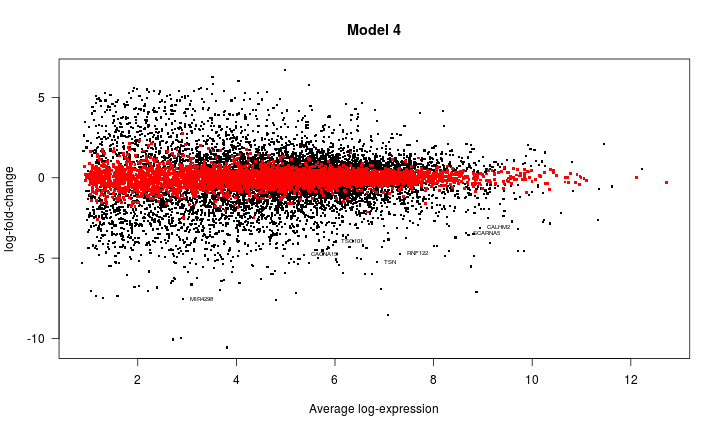
\includegraphics[width=\linewidth]{maPlot-1}
\caption{MA-plot for the model 4, adjusting the known covariate TSS and unkwnown covariates using SVA}
\label{fig:MAplot}
\end{figure}

From the last model, a factorial design was performed in order to analyse the interaction between \textit{type} (tumor or normal) and \textit{TSS}, concretely with BG and BK. It was not successful, as there were not genes which were clearly differentially expressed in only one 	of them. For future analyses, it could be interesting to analyse the interaction between other possible sources of unwanted variation such as \textit{histological diagnosis}, as it has been seen in several studies that there are genes clearly differentially expressed between serous and endometroid tumors \citep{Getz2013}.

The more complete model is the last one, as it includes to an adjusted model for mean-variance relationship the adjustment to variability of known and unknown covariates. The number of differentially expressed genes increases importantly in this model with respect to the others. But as in previous steps we removed any possible sources of variation, the more variables that we put in our model, the fewer degrees of freedom it has, and thus the less statistical power that is has. Therefore, this model is the one used in the posterior Functional Enrichment analysis.

\subsection{Functional Enrichment: The Gene Ontology analysis}

In the \textit{table X} we can see the list of the 10 most significantly differentially expressed pathways in uterine tumour tissue, taking the ordered goresults obtained from the final set of DEgenes. 

\begin{table}
\centering
\caption{Ten most significant gene ontologies found in the Functional Enrichment analysis}
\begin{tableminipage}{\textwidth}
 \begin{tabular}{|| c c c c c||} 
 \hline
 \textbf{GOBPID} & \textbf{Pvalue} & \textbf{OddsRatio} & \textbf{Excount} & \textbf{Count} \\ [0.5ex] 
 \hline\hline
 GO:0010762 & 0.0068 & Inf & 8.8567 & 13 \\
 \multicolumn{5}{||c||}{regulation of fibroblast migration} \\ 
 \hline
 GO:1903543 & 0.0100 & Inf & 8.1754 & 12 \\
 \multicolumn{5}{||c||}{positive regulation of exosomal secretion} \\ 
 \hline
 GO:0007213 & 0.0146 & Inf & 7.4941 & 11 \\
 \multicolumn{5}{||c||}{G-protein coupled acetylcholine receptor signaling pathway} \\ 
 \hline
 GO:0032735 & 0.0146 & Inf & 7.4941 & 11 \\
 \multicolumn{5}{||c||}{positive regulation of interleukin-12 production} \\ 
  \hline
 GO:0046636 & 0.0146 & Inf & 7.4941 & 11 \\
 \multicolumn{5}{||c||}{negative regulation of alpha-beta T cell activation} \\ 
  \hline
 GO:0071380 & 0.0146 & Inf & 7.4941 & 11 \\
 \multicolumn{5}{||c||}{cellular response to prostaglandin E stimulus} \\ 
  \hline
 GO:0010842 & 0.0215 & Inf & 6.8128 & 10 \\
 \multicolumn{5}{||c||}{retina layer formation} \\ 
  \hline
 GO:0036092 & 0.0215 & Inf & 6.8128 & 10 \\
 \multicolumn{5}{||c||}{phosphatidylinositol-3-phosphate biosynthetic process} \\ 
  \hline
 GO:0045986 & 0.0215 & Inf & 6.8128 & 10 \\
 \multicolumn{5}{||c||}{negative regulation of smooth muscle contraction} \\ 
  \hline
 GO:0007063 &  0.0316 & Inf & 6.1316 & 9 \\
 \multicolumn{5}{||c||}{regulation of sister chromatid cohesion} \\ 
 \hline
\end{tabular}
  \label{tab:shape-functions}
\end{tableminipage}
\end{table}

Taking those 10 top GO terms, our analysis identified nine functional groups which could be, directly or indirectly, involved in endometrial cancer. One of them seems to be a functional group specific from our cancer type, while the others don't. Another one, related to the retina formation, does not seem to be biochemically related to the UCEC. 

Between the eight groups that can be related to cancer we find:
\begin{itemize}
  \item \textbf{Regulation of fibroblast migration}, which is directly related with tissue damage, and therefore, with tumors. Fibroblasts are considered to have a key role in the malignant progression of cancer and represent an important target in endometrial cancer research, as it has been demonstrated in some current articles (1,2,3).
  \item \textbf{Regulation of sister chromatid cohesion}, as it has been proved that aberrant sister chromatid cohesion causes instability and contributes to the development of cancer (5). Several studies have targeted candidate chromosome instability genes in order to treat endometrial cancer (4).
  \item \textbf{Positive regulation of exosomal secretion}, which is fundamental due to the increasing evidence that tumor cells release excessive amount of exosomes (10).
  \item \textbf{Regulation of interleukin-12 production} and \textbf{alpha-beta T cell activation} are clearly part of the development of the immune response against the tumor (11,12), and therefore, they are differentially expressed in comparison with normal samples. 
  \item \textbf{G-protein coupled receptor pathway} or \textbf{phosphatidyli-nositol-3-phosphate biosyntesis} are two cases belonging to signaling pathways, also affected by cancer development (7,8).
\end{itemize}

There is one group identified between the top ten differentially expressed functional groups which has been directly related with endometrial cancer: \textbf{negative regulation of smooth muscle contraction}. This is because fibroids, which are benign tumours of smooth muscle, are believed to alter muscular contraction of uterus (13). However, there is not much investigation in this direction.

It is also important to remark that there are two differentially expressed genes known to have important roles in endometrial cancer which are part of two of the top ten differentially expressed functional groups. The first is PIK3C2A, which is part of the Phosphatidylinositol-3-phosphate biosynthetic process, and has an established role in the pathogenesis of serous endometrial cancer (5). The second is CTNNB1, in regulation of sister chromatid cohesion, a gene with an unusually high frequency of mutations in endometroid tumors (52\%) (6). \\

The differential expression and functional enrichment analysis have provided an interesting perspective of the endometrial cancer, remarking the most important genes and pathways which suffer changes during the disease, and raising hypotheses about how they could affect to its advance. 

\section*{Additional guidelines}

\subsection*{Numbers} In the text, write out numbers nine or less except as part of a date, a fraction or decimal, a percentage, or a unit of measurement. Use Arabic numbers for those larger than nine, except as the first word of a sentence; however, try to avoid starting a sentence with such a number.

\subsection*{Units} Use abbreviations of the customary units of measurement only when they are preceded by a number: "3 min" but "several minutes". Write "percent" as one word, except when used with a number: "several percent" but "75\%." To indicate temperature in centigrade, use ° (for example, 37°); include a letter after the degree symbol only when some other scale is intended (for example, 45°K).

\subsection*{Nomenclature and Italicization} Italicize names of organisms even when  when the species is not indicated.  Italicize the first three letters of the names of restriction enzyme cleavage sites, as in HindIII. Write the names of strains in roman except when incorporating specific genotypic designations. Italicize genotype names and symbols, including all components of alleles, but not when the name of a gene is the same as the name of an enzyme. Do not use "+" to indicate wild type. Carefully distinguish between genotype (italicized) and phenotype (not italicized) in both the writing and the symbolism.

\section*{In-text Citations}

Add citations using the \verb|\citep{}| command, for example \citep{neher2013genealogies} or for multiple citations, \citep{neher2013genealogies, rodelsperger2014characterization}

\section*{Examples of Article Components}
\label{sec:examples}

The sections below show examples of different header levels, which you can use in the primary sections of the manuscript (Results, Discussion, etc.) to organize your content.

\section*{First level section header}

Use this level to group two or more closely related headings in a long article.

\subsection*{Second level section header}

Second level section text.

\subsubsection*{Third level section header:}

Third level section text. These headings may be numbered, but only when the numbers must be cited in the text. 

\section*{Figures and Tables}

Figures and Tables should be labelled and referenced in the standard way using the \verb|\label{}| and \verb|\ref{}| commands.

\subsection*{Sample Figure}

Figure \ref{fig:spectrum} shows an example figure.

\begin{figure}[htbp]
\centering
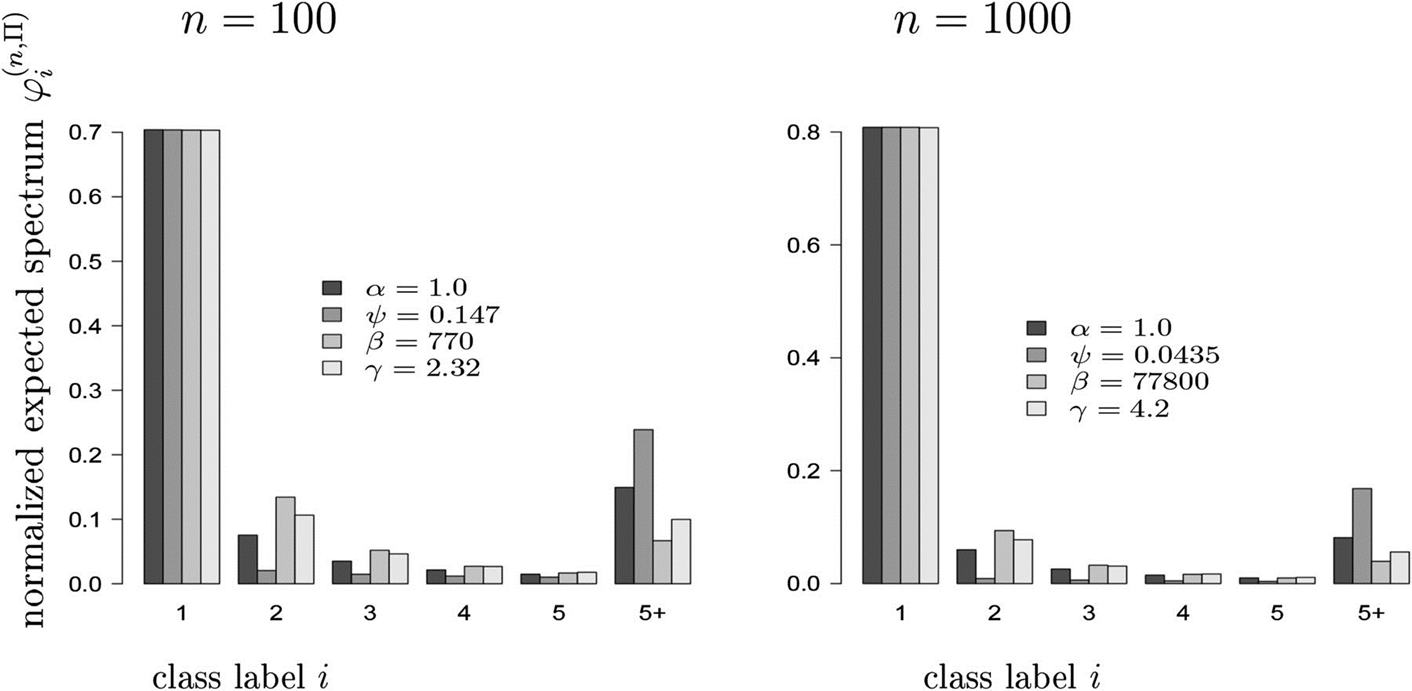
\includegraphics[width=\linewidth]{example-figure}
\caption{Example figure from \url{10.1534/genetics.114.173807}. Please include your figures in the manuscript for the review process. You can upload figures to Overleaf via the Project menu. Upon acceptance, we'll ask for your figure files to be uploaded in any of the following formats: TIFF (.tiff), JPEG (.jpg), Microsoft PowerPoint (.ppt), EPS (.eps), or Adobe Illustrator (.ai).  Images should be a minimum of 300 dpi in resolution and 500 dpi minimum if line art images.  RGB, CMYK, and Grayscale are all acceptable. Halftones should be high contrast with sharp detail, because some loss of detail and contrast is inevitable in the production process. Figures should be 10-20 cm in width and 1-25 cm in height. Graph axes must be exactly perpendicular and all lines of equal density.
Label multiple figure parts with A, B, etc. in bolded type, and use Arrows and numbers to draw attention to areas you want to highlight. Legends should start with a brief title and should be a self-contained description of the content of the figure that provides enough detail to fully understand the data presented. All conventional symbols used to indicate figure data points are available for typesetting; unconventional symbols should not be used. Italicize all mathematical variables (both in the figure legend and figure) , genotypes, and additional symbols that are normally italicized.  
}%
\label{fig:spectrum}
\end{figure}

\subsection*{Sample Video}

Figure \ref{video:spectrum} shows how to include a video in your manuscript.

\begin{figure}[htbp]
\centering
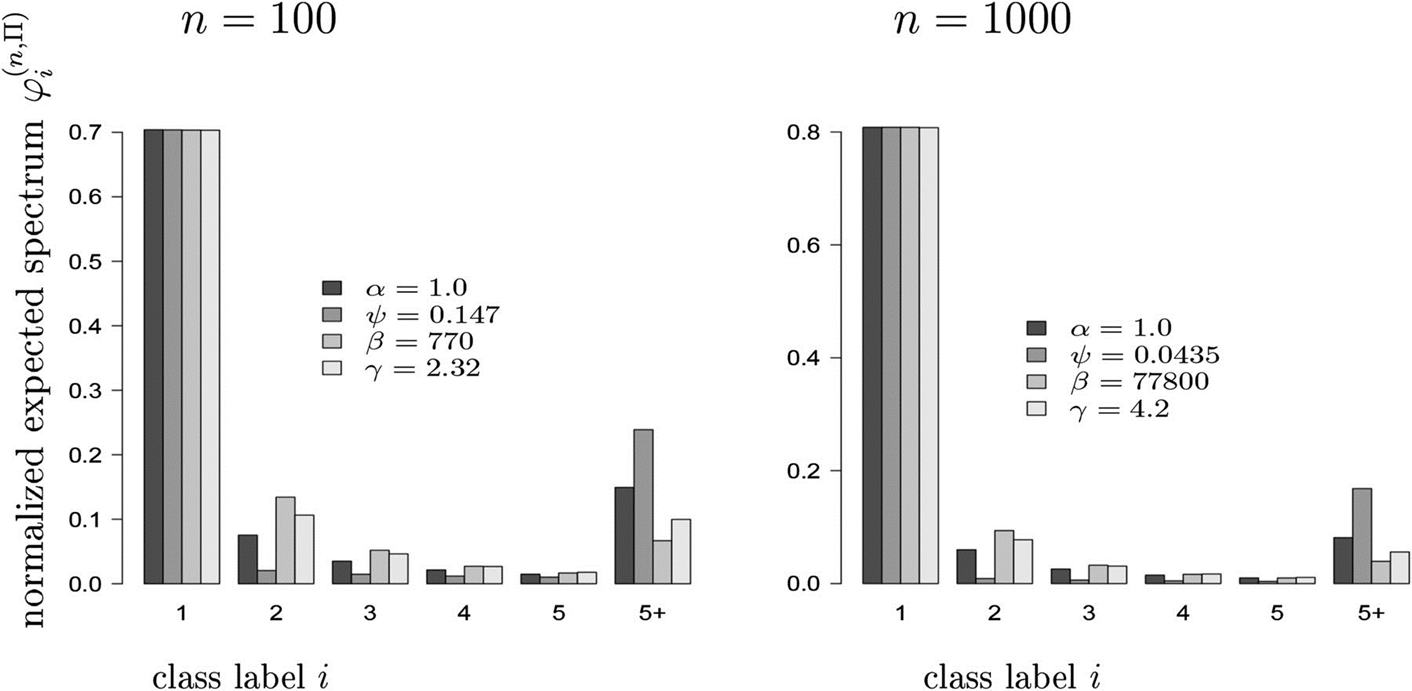
\includegraphics[width=\linewidth]{example-figure}
\caption{Example movie (the figure file above is used as a placeholder for this example). \textit{GENETICS} supports video and movie files that can be linked from any portion of the article - including the abstract. Acceptable formats include .asf, avi, .wav, and all types of Windows Media files.   
}%
\label{video:spectrum}
\end{figure}


\subsection*{Sample Table}

Table \ref{tab:shape-functions} shows an example table. Avoid shading, color type, line drawings, graphics, or other illustrations within tables. Use tables for data only; present drawings, graphics, and illustrations as separate figures. Histograms should not be used to present data that can be captured easily in text or small tables, as they take up much more space.  

Tables numbers are given in Arabic numerals. Tables should not be numbered 1A, 1B, etc., but if necessary, interior parts of the table can be labeled A, B, etc. for easy reference in the text.  


\begin{table*}[htbp]
\centering
\caption{\bf Students and their grades}
\begin{tableminipage}{\textwidth}
\begin{tabularx}{\textwidth}{XXXX}
\hline
Student & Grade\footnote{This is an example of a footnote in a table. Lowercase, superscript italic letters (a, b, c, etc.) are used by default. You can also use *, **, and *** to indicate conventional levels of statistical significance, explained below the table.} & Rank & Notes \\
\hline
Alice & 82\% & 1 & Performed very well.\\
Bob & 65\% & 3 & Not up to his usual standard.\\
Charlie & 73\% & 2 & A good attempt.\\
\hline
\end{tabularx}
  \label{tab:shape-functions}
\end{tableminipage}
\end{table*}

\section*{Sample Equation}

Let $X_1, X_2, \ldots, X_n$ be a sequence of independent and identically distributed random variables with $\text{E}[X_i] = \mu$ and $\text{Var}[X_i] = \sigma^2 < \infty$, and let
\begin{equation}
S_n = \frac{X_1 + X_2 + \cdots + X_n}{n}
      = \frac{1}{n}\sum_{i}^{n} X_i
\label{eq:refname1}
\end{equation}
denote their mean. Then as $n$ approaches infinity, the random variables $\sqrt{n}(S_n - \mu)$ converge in distribution to a normal $\mathcal{N}(0, \sigma^2)$.

\bibliography{IEO_UCEC}

\end{document}